\section{步长的选择}
\label{sec:smooth-step-size}

现在固定当前点$\bm{x}$和一个下降方向$\bm{d}$，只决定走多远。记$\bm{g}=\nabla f(\bm{x})$，并把目标限制到这条射线上：
\begin{equation}
 \phi(\alpha)=f(\bm{x}+\alpha\bm{d}),\qquad \alpha\geq0.
 \label{eq:smooth-phi}
\end{equation}
由链式法则，
\[
 \phi'(\alpha)=\langle\nabla f(\bm{x}+\alpha\bm{d}),\bm{d}\rangle,\qquad \phi'(0)=\langle\bm{g},\bm{d}\rangle<0.
\]

候选步长满足什么条件，就可以接受？这个问题有三种回答，区别在于事先要知道什么、每一步要多算什么。固定步长事先靠$L$定好，运行时什么也不检验。回溯线搜索不需要$L$，用函数值检验每个候选。Wolfe条件再加上对方向导数的检验，换来更强的保证。

在二次目标上，$\phi$是一条抛物线，三种规则都可以写成步长的区间。设$f(\bm{x})=\frac12\bm{x}^\top\bm{H}\bm{x}$，$\bm{H}$对称正定，$\langle\bm{d},\bm{H}\bm{d}\rangle>0$。将$\phi$展开，得到
\[
 \phi(\alpha)=\phi(0)+\alpha\phi'(0)+\frac{\alpha^2}{2}\langle\bm{d},\bm{H}\bm{d}\rangle.
\]
它的最低点记作
\begin{equation}
 \alpha_{\mathrm{e}}=\frac{-\phi'(0)}{\langle\bm{d},\bm{H}\bm{d}\rangle}.
 \label{eq:smooth-exact-quadratic}
\end{equation}

用$\alpha_{\mathrm{e}}$改写，后面反复要用的两个式子是
\begin{equation}
 \begin{gathered}
 \phi(\alpha)=\phi(0)+\alpha\phi'(0)\Bigl(1-\frac{\alpha}{2\alpha_{\mathrm{e}}}\Bigr),\\
 \phi'(\alpha)=\phi'(0)\Bigl(1-\frac{\alpha}{\alpha_{\mathrm{e}}}\Bigr).
 \end{gathered}
 \label{eq:smooth-quadratic-line}
\end{equation}

例~\eqref{eq:smooth-running}从$\bm{x}^{(0)}$沿$\bm{d}=-\bm{g}^{(0)}=(-9,-9)$走时，下面三个数在本节一直用到：
\[
 \phi'(0)=-162,\qquad \langle\bm{d},\bm{H}\bm{d}\rangle=810,\qquad \alpha_{\mathrm{e}}=\frac15.
\]
这条线上的目标是
\[
 \phi(\alpha)=45-162\alpha+405\alpha^2.
\]

\subsection{固定步长}
\label{sec:smooth-fixed-step}

\paragraph{负梯度方向}
先看最简单的情形：$\bm{d}=-\bm{g}$，步长是事先定好的常数。在下降引理~\eqref{eq:smooth-descent-lemma}中取$\bm{p}=-\alpha\bm{g}$，得到
\begin{equation}
 f(\bm{x}-\alpha\bm{g})\leq f(\bm{x})-\alpha\Bigl(1-\frac{L\alpha}{2}\Bigr)\lVert\bm{g}\rVert_2^2.
 \label{eq:smooth-gd-step}
\end{equation}

括号前的$\alpha$是沿坡度得到的收益，括号里的$L\alpha/2$是弯曲带来的折扣。只要$0<\alpha<2/L$，保证的下降量就是正的。保证的下降量是$\alpha$的二次函数，在$\alpha=1/L$处最大，值为$\lVert\bm{g}\rVert_2^2/(2L)$，这就是式~\eqref{eq:smooth-model-min}。

图~\ref{fig:smooth-step-upper-bound}在例~\eqref{eq:smooth-running}上比较上界与真实目标。$L=9$，$\lVert\bm{g}^{(0)}\rVert_2^2=162$，上界是
\[
 45-162\alpha+729\alpha^2.
\]
取$\alpha=1/L=1/9$时，上界为$36$，真实值为$32$。上界在$\alpha=2/L$处回到$45$，真实目标却要到$\alpha=0.4$才回到$45$。

这个差别来自方向。这条线上目标的曲率是$810/162=5$，小于最坏方向的$9$。所以$2/L$并不是这个方向上真实的界限，而是对所有点、所有方向都安全的界限。

\begin{BookInlineFigure}
  \centering
  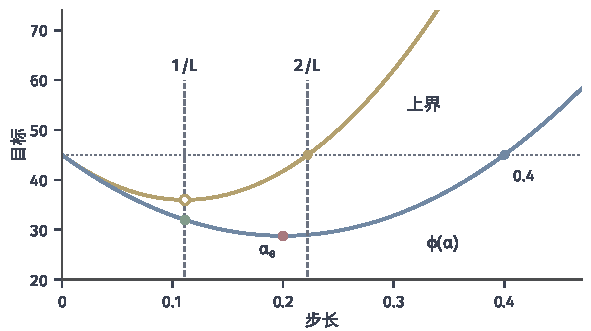
\includegraphics[width=100mm]{figures/05-optimization/02-smooth-optimization/matplotlib/smooth-step-upper-bound/figure.pdf}
  \caption{沿负梯度的一维剖面，例~\eqref{eq:smooth-running}，$\bm{x}^{(0)}=(9,1)$。蓝线是真实的$\phi(\alpha)$，黄线是下降引理的上界，点线是当前高度$45$。上界的最低点在$1/L$，回到$45$的位置是$2/L$；真实目标的最低点是红点$\alpha_{\mathrm{e}}=0.2$，回到$45$的位置是$0.4$。绿点是$\alpha=1/L$时的真实值，它低于同一步长的上界值（空心点）。}
  \label{fig:smooth-step-upper-bound}
\end{BookInlineFigure}

\paragraph{界限$2/L$在最坏方向上是紧的}
一元二次目标$f(x)=\frac{L}{2}x^2$说明，范围不能放宽。更新$x^+=x-\alpha Lx=(1-\alpha L)x$，乘数的绝对值小于$1$当且仅当$0<\alpha<2/L$。$\alpha=2/L$时乘数是$-1$，迭代来回跳；$\alpha>2/L$时迭代发散。

对二次目标，每个特征方向各自按这个规律变化。例~\eqref{eq:smooth-running}中$\bm{H}$是对角阵，固定步长的迭代逐分量写出来是
\[
 x_1^{(t+1)}=(1-\alpha)x_1^{(t)},\qquad x_2^{(t+1)}=(1-9\alpha)x_2^{(t)}.
\]
图~\ref{fig:smooth-fixed-paths}比较三个步长。$\alpha=1/9$时第二个乘数为零，一步消去最陡的分量，此后沿平坦方向每步只缩小到$8/9$。$\alpha=1/5$时两个乘数是$0.8$和$-0.8$，大小相同，路径锯齿前进。$\alpha=1/4$超过了$2/L=2/9$，第二个乘数是$-1.25$，$x_2$振荡发散。

\begin{BookInlineFigure}
  \centering
  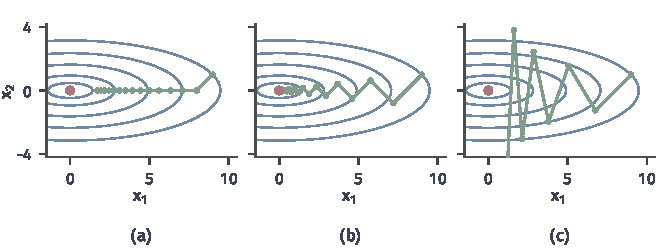
\includegraphics[width=112mm]{figures/05-optimization/02-smooth-optimization/matplotlib/smooth-fixed-paths/figure.pdf}
  \caption{例~\eqref{eq:smooth-running}上固定步长的梯度下降路径，绿点是迭代点，红点是最优解。(a)$\alpha=1/9$，乘数为$8/9$和$0$。(b)$\alpha=1/5$，乘数为$0.8$和$-0.8$。(c)$\alpha=1/4>2/L$，乘数为$0.75$和$-1.25$，路径沿$x_2$方向越摆越大。}
  \label{fig:smooth-fixed-paths}
\end{BookInlineFigure}

\paragraph{已知上界时怎样选}
若手里有一个上界$\hat{L}\geq L$，取$\alpha=1/\hat{L}$总是安全的。代入式~\eqref{eq:smooth-gd-step}，并用$L/\hat{L}\leq1$，得到
\[
 f(\bm{x})-f(\bm{x}-\alpha\bm{g})\geq\frac{1}{2\hat{L}}\lVert\bm{g}\rVert_2^2.
\]
上界放大几倍，保证的下降量就缩小几倍，这是高估的代价。低估的代价可能更严重：$\hat{L}<L/2$时$\alpha>2/L$，最坏方向上会发散。例~\eqref{eq:smooth-running}若误取$\hat{L}=4$，得到的恰是图~\ref{fig:smooth-fixed-paths}(c)。

固定步长的运行过程只有一步：算梯度，走$\alpha$，再算梯度。它每轮只读一次梯度，不计算函数值，也不做任何检验，这是它最大的优点。目标只在下水平集上有常数时，引理~\ref{lem:smooth-sublevel}说明用$\bm{S}=\{f\leq f(\bm{x}^{(0)})\}$上的$L$就够了；每步下降保证迭代留在$\bm{S}$内，同一个常数可以一直用。

\paragraph{一般下降方向}
后面各章的方向不一定是负梯度，上面的区间不能照搬。在下降引理中取$\bm{p}=\alpha\bm{d}$，得到
\begin{equation}
 f(\bm{x}+\alpha\bm{d})\leq f(\bm{x})+\alpha\langle\bm{g},\bm{d}\rangle+\frac{L\alpha^2}{2}\lVert\bm{d}\rVert_2^2.
 \label{eq:smooth-direction-bound}
\end{equation}

右端是$\alpha$的二次函数。它低于$f(\bm{x})$的范围、取最小值的步长分别是
\begin{equation}
 0<\alpha<\frac{2\lvert\langle\bm{g},\bm{d}\rangle\rvert}{L\lVert\bm{d}\rVert_2^2},\qquad
 \alpha=\frac{\lvert\langle\bm{g},\bm{d}\rangle\rvert}{L\lVert\bm{d}\rVert_2^2}.
 \label{eq:smooth-direction-range}
\end{equation}

代入后，一步保证的下降量可以用$\bm{d}$与$-\bm{g}$的夹角$\theta$表示：
\begin{equation}
 \frac{\langle\bm{g},\bm{d}\rangle^2}{2L\lVert\bm{d}\rVert_2^2}=\frac{\cos^2\theta}{2L}\lVert\bm{g}\rVert_2^2,
 \qquad\cos\theta=\frac{\lvert\langle\bm{g},\bm{d}\rangle\rvert}{\lVert\bm{g}\rVert_2\lVert\bm{d}\rVert_2}.
 \label{eq:smooth-cos-decrease}
\end{equation}

式~\eqref{eq:smooth-direction-range}含有方向的长度和方向导数，这两点都有具体后果。先看长度。把方向放大$10$倍，$\bm{d}=-10\bm{g}^{(0)}$，再取$\alpha=1/L=1/9$，实际位移是$-\frac{10}{9}\bm{g}^{(0)}$，于是
\[
 \bm{x}^{(1)}=(9,1)-10(1,1)=(-1,-9),\qquad f(\bm{x}^{(1)})=365.
\]
目标从$45$涨到$365$。图~\ref{fig:smooth-direction-scale}(a)的虚线正是这种情形。步长的单位包含了方向的长度，$1/L$只适用于$\bm{d}=-\bm{g}$这一个尺度。

\begin{BookInlineFigure}
  \centering
  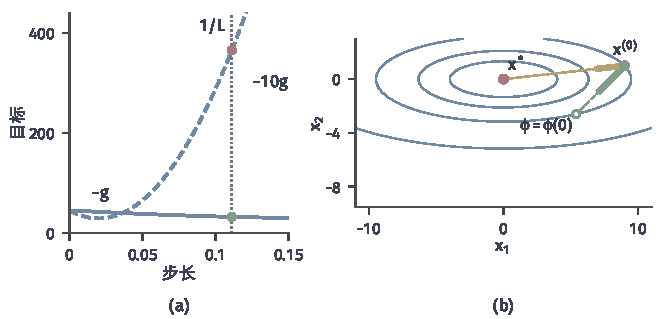
\includegraphics[width=112mm]{figures/05-optimization/02-smooth-optimization/matplotlib/smooth-direction-scale/figure.pdf}
  \caption{一般方向不能照搬$\alpha<2/L$。(a)沿$-\bm{g}$（实线）与$-10\bm{g}$（虚线）的目标剖面，同样取$\alpha=1/L$，前者到$32$，后者到$365$。(b)从$\bm{x}^{(0)}$出发的两个方向：绿色$-\bm{g}$，黄色$-\bm{H}^{-1}\bm{g}$。粗线段是式~\eqref{eq:smooth-direction-range}保证下降的范围，虚线延伸到真实目标回到起始高度或到达最低点的位置。}
  \label{fig:smooth-direction-scale}
\end{BookInlineFigure}

再看方向导数。取$\bm{d}=(-1,0.9)$，它几乎贴着等高线，$\langle\bm{g}^{(0)},\bm{d}\rangle=-0.9$，$\lVert\bm{d}\rVert_2^2=1.81$，由式~\eqref{eq:smooth-cos-decrease}，保证的下降量是
\[
 \frac{0.81}{2\cdot9\cdot1.81}\approx0.025,
\]
而负梯度方向是$9$。方向虽然严格下降，贴着等高线走，保证的进展几乎没有。

第三个例子说明上界有时过于悲观。$\bm{d}=-\bm{H}^{-1}\bm{g}^{(0)}=(-9,-1)$时，式~\eqref{eq:smooth-direction-range}的范围是
\[
 0<\alpha<\frac{2\cdot90}{9\cdot82}\approx0.244.
\]
但这个方向直指最优解，$\alpha=1$一步到位。上界用的是最陡方向的曲率$9$，这条线上的实际曲率却只有
\[
 \frac{\langle\bm{d},\bm{H}\bm{d}\rangle}{\lVert\bm{d}\rVert_2^2}=\frac{90}{82}\approx1.1.
\]
图~\ref{fig:smooth-direction-scale}(b)的黄色粗线段远短于黄色虚线，差的就是这个比值。

这三个例子都说明，固定步长依赖对$L$和方向尺度的先验知识。下一小节改用实际目标值检验候选。

\subsection{回溯线搜索}
\label{sec:smooth-backtracking}

\paragraph{主要思想}
不知道$L$时，不妨先迈一大步，看看真实高度是否令人满意；不满意就退回来，迈小一些。这里的关键是“满意”的标准。只要求$\phi(\alpha)<\phi(0)$是不够的，后面会看到，这样的下降可能小到不产生进展。

合理的标准是把实际下降与一阶预测比较。走$\alpha$时，线性预测的下降量是$-\alpha\phi'(0)$。我们要求实际下降不少于预测的固定比例。这和记账相似：线性预测是承诺的收益，实际下降是到账的收益，至少到账一定比例才算数。

\begin{definition}[Armijo条件]
\label{def:smooth-armijo}
设$\langle\bm{g},\bm{d}\rangle<0$，$c_1\in(0,1)$。若步长$\alpha>0$满足
\begin{equation}
 f(\bm{x}+\alpha\bm{d})\leq f(\bm{x})+c_1\alpha\langle\bm{g},\bm{d}\rangle,
 \label{eq:smooth-armijo}
\end{equation}
就说它满足\term{Armijo条件}（Armijo condition），也称\term{充分下降条件}（sufficient decrease condition）。
\end{definition}

条件的右端是从$(0,\phi(0))$出发、斜率为$c_1\phi'(0)$的直线，它比切线平缓。Armijo条件要求曲线落在这条直线下方。$c_1$的两个端点都不能取：$c_1=0$退化成只要求下降，$c_1=1$时直线就是切线，而凸的$\phi$永远不低于切线，没有步长可以通过。实践中常取很小的值，如$c_1=10^{-4}$\scite{math-nocedal2006numerical}。

由式~\eqref{eq:smooth-quadratic-line}，二次目标上的Armijo条件化为$1-\alpha/(2\alpha_{\mathrm{e}})\geq c_1$，也就是
\begin{equation}
 0<\alpha\leq2(1-c_1)\alpha_{\mathrm{e}}.
 \label{eq:smooth-armijo-quadratic}
\end{equation}
例中取$c_1=0.1$，可接受的步长是$(0,0.36]$，如图~\ref{fig:smooth-armijo}中的绿色线段。

\begin{BookInlineFigure}
  \centering
  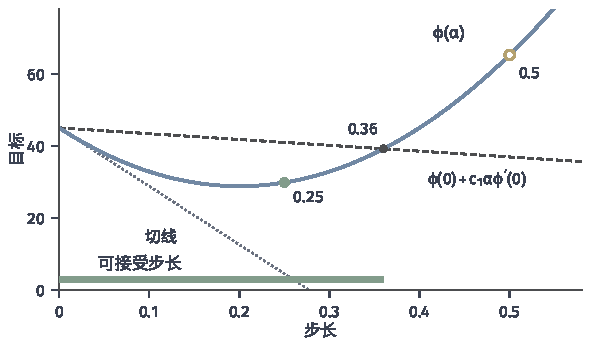
\includegraphics[width=100mm]{figures/05-optimization/02-smooth-optimization/matplotlib/smooth-armijo/figure.pdf}
  \caption{Armijo条件，例~\eqref{eq:smooth-running}第一轮，$c_1=0.1$。蓝线是$\phi(\alpha)$，点线是切线，深灰虚线是斜率为$c_1\phi'(0)$的检验直线，曲线在它下方的步长（绿色线段）$(0,0.36]$可接受。回溯从$\alpha=1$开始（$\phi(1)=288$，在图外），$\alpha=0.5$被拒绝（空心点），$\alpha=0.25$通过（绿点）。}
  \label{fig:smooth-armijo}
\end{BookInlineFigure}

这样的做法称为\term{回溯线搜索}（backtracking line search）：从初始试探步长$\alpha_0$开始，不满足式~\eqref{eq:smooth-armijo}就乘以缩减因子$\rho\in(0,1)$，第一个通过的步长就是结果。下面的定理回答这个过程为什么会停，以及停在多大的步长上。

\begin{theorem}[回溯的终止与步长下界]
\label{thm:smooth-backtracking}
设$f$在$\bm{x}$处可微，$\langle\bm{g},\bm{d}\rangle<0$，$c_1,\rho\in(0,1)$，$\alpha_0>0$。则回溯经有限次试探后终止。

进一步设$\nabla f$在线段$\{\bm{x}+s\bm{d}:s\in[0,\alpha_0]\}$上以常数$L>0$满足式~\eqref{eq:smooth-lipschitz}，并记
\begin{equation}
 \bar{\alpha}=\frac{2(1-c_1)\lvert\langle\bm{g},\bm{d}\rangle\rvert}{L\lVert\bm{d}\rVert_2^2}.
 \label{eq:smooth-armijo-threshold}
\end{equation}
则$(0,\alpha_0]$中不超过$\bar{\alpha}$的步长都满足Armijo条件，接受的步长$\alpha$和试探次数$n$满足
\begin{equation}
 \alpha\geq\min\{\alpha_0,\rho\bar{\alpha}\},\qquad
 n\leq1+\Bigl\lceil\log_{1/\rho}\frac{\alpha_0}{\bar{\alpha}}\Bigr\rceil_+,
 \label{eq:smooth-backtracking-bounds}
\end{equation}
其中$\lceil a\rceil_+=\max\{\lceil a\rceil,0\}$。一步的下降量满足
\begin{equation}
 f(\bm{x})-f(\bm{x}+\alpha\bm{d})\geq c_1\min\{\alpha_0,\rho\bar{\alpha}\}\lvert\langle\bm{g},\bm{d}\rangle\rvert.
 \label{eq:smooth-backtracking-decrease}
\end{equation}
\end{theorem}

\begin{proof}
先证终止。由可微性，当$\alpha\downarrow0$时
\[
 \frac{\phi(\alpha)-\phi(0)}{\alpha}\to\phi'(0).
\]
因为$\phi'(0)<0$且$c_1<1$，所以$\phi'(0)<c_1\phi'(0)$。于是存在$\alpha'>0$，使$\alpha\in(0,\alpha']$时差商小于$c_1\phi'(0)$，这正是式~\eqref{eq:smooth-armijo}。试探步长$\alpha_0\rho^{j}$趋于零，有限步后落入$(0,\alpha']$。

再证定量部分。设$\alpha\in(0,\alpha_0]$，$\alpha\leq\bar{\alpha}$。线段上的Lipschitz条件使式~\eqref{eq:smooth-direction-bound}成立。由$\alpha\leq\bar{\alpha}$得到
\[
 \frac{L\alpha}{2}\lVert\bm{d}\rVert_2^2\leq(1-c_1)\lvert\langle\bm{g},\bm{d}\rangle\rvert.
\]
代入式~\eqref{eq:smooth-direction-bound}的最后一项，得到
\[
 f(\bm{x}+\alpha\bm{d})\leq f(\bm{x})+\alpha\langle\bm{g},\bm{d}\rangle+\alpha(1-c_1)\lvert\langle\bm{g},\bm{d}\rangle\rvert.
\]
由$\langle\bm{g},\bm{d}\rangle<0$，右端等于式~\eqref{eq:smooth-armijo}的右端。

若$\alpha_0$直接通过，则$\alpha=\alpha_0$。否则，被接受步长的上一次试探$\alpha/\rho$未通过，由刚证的结论$\alpha/\rho>\bar{\alpha}$，所以$\alpha>\rho\bar{\alpha}$。这得到步长下界。

第$j$次试探的步长是$\alpha_0\rho^{j-1}$，它一旦不超过$\bar{\alpha}$就一定通过，这要求$j-1\geq\log_{1/\rho}(\alpha_0/\bar{\alpha})$，试探次数的上界由此得出。把步长下界代入式~\eqref{eq:smooth-armijo}，即得式~\eqref{eq:smooth-backtracking-decrease}。
\end{proof}

定理中各条件的作用可以分开看。下降方向是必需的：若$\phi'(0)>0$，式~\eqref{eq:smooth-armijo}对所有充分小的$\alpha$都不成立，回溯不会在小步长上停下来。终止只用到当前点的可微性，算法也不需要知道$L$。$L$只出现在分析里，用来定量说明步长不会太小。

这里的$L$只要覆盖试探过的线段，这就是局部光滑性足够的原因。取$f(x)=x^4$，它没有全局的$L$，从$x=1.5$出发，$d=-13.5$，$c_1=0.1$，$\rho=1/2$，$\alpha_0=1$。试探点和目标值依次是
\[
 \begin{aligned}
 \alpha=1:&\quad x=-12,\quad f=20736,\\
 \alpha=\tfrac12:&\quad x=-5.25,\quad f\approx759.7,\\
 \alpha=\tfrac14:&\quad x=-1.875,\quad f\approx12.36,\\
 \alpha=\tfrac18:&\quad x=-0.1875,\quad f\approx0.0012.
 \end{aligned}
\]
最后一次的右端是$5.0625-0.1\cdot\frac18\cdot182.25\approx2.78$，条件满足。用固定步长时必须事先想清楚区域和常数，回溯把这些问题都交给了实际的函数值。

\paragraph{计算过程}
下面用例~\eqref{eq:smooth-running}走一遍，方向取负梯度，这也是下一章梯度下降法使用的形式。

\needspace{6\baselineskip}
\paragraph{变量}
\begin{itemize}
 \item $\bm{x}\in\mathbb{R}^n$：当前点；$\bm{g}\in\mathbb{R}^n$：当前梯度；$\bm{d}\in\mathbb{R}^n$：方向。
 \item $f_{\mathrm{cur}}$：当前目标值；$\sigma=\langle\bm{g},\bm{d}\rangle$：方向导数，是一个负数。
 \item $\alpha$：当前试探步长；$c_1,\rho,\alpha_0$：Armijo常数、缩减因子、初始试探步长。
 \item $\varepsilon$：梯度容差。
\end{itemize}

\paragraph{初始化}
取定初始点，算出它的目标值和梯度。例中$\bm{x}=(9,1)$，参数和初值是
\[
 c_1=0.1,\quad\rho=0.5,\quad\alpha_0=1,\quad\varepsilon=10^{-3},
\]
\[
 f_{\mathrm{cur}}=45,\quad\bm{g}=(9,9).
\]

\needspace{6\baselineskip}
\paragraph{每轮更新}
\begin{enumerate}
 \item 计算方向$\bm{d}=-\bm{g}$和方向导数$\sigma=-\lVert\bm{g}\rVert_2^2$。令$\alpha\leftarrow\alpha_0$。

 例中第一轮$\bm{d}=(-9,-9)$，$\sigma=-162$，$\alpha=1$。

 \item 计算试探点$\bm{x}+\alpha\bm{d}$及其目标值，按式~\eqref{eq:smooth-armijo}与$f_{\mathrm{cur}}+c_1\alpha\sigma$比较。不满足就令$\alpha\leftarrow\rho\alpha$，重复这一步。

 例中第一轮的三次试探依次是
 \[
 \begin{aligned}
 \alpha=1:&\quad(0,-8),\quad f=288>28.8,\\
 \alpha=0.5:&\quad(4.5,-3.5),\quad f=65.25>36.9,\\
 \alpha=0.25:&\quad(6.75,-1.25),\quad f=29.8125\leq40.95.
 \end{aligned}
 \]
 第三次通过。

 \item 接受试探点，更新$\bm{x}$、$f_{\mathrm{cur}}$，计算新梯度。

 例中得到
 \[
 \bm{x}=(6.75,-1.25),\quad f_{\mathrm{cur}}=29.8125,\quad\bm{g}=(6.75,-11.25).
 \]

 \item 若$\lVert\bm{g}\rVert_2\leq\varepsilon$，停止；否则回到第1步。

 例中$\lVert\bm{g}\rVert_2\approx13.12$，继续。第二轮$\sigma=-172.125$，试探如下：
 \[
 \begin{aligned}
 \alpha=1:&\quad(0,10),\quad f=450>12.6,\\
 \alpha=0.5:&\quad(3.375,4.375),\quad f\approx91.83>21.21,\\
 \alpha=0.25:&\quad(5.0625,1.5625),\quad f\approx23.80\leq25.51.
 \end{aligned}
 \]
\end{enumerate}

后面几轮的结果列在表~\ref{tab:smooth-backtrack-run}中，路径见图~\ref{fig:smooth-backtrack-path}。第一轮接受的$0.25$超过了固定步长的安全上限$2/L=2/9$，这正是检验真实函数值带来的好处。

\begin{BookInlineTable}
  \centering
  \begin{tabular}{@{}rrrrrrr@{}}
    \toprule
    $t$ & $x_1^{(t)}$ & $x_2^{(t)}$ & $f(\bm{x}^{(t)})$ & $\lVert\bm{g}^{(t)}\rVert_2$ & 试探次数 & $\alpha^{(t)}$\\
    \midrule
    0 & 9.000 & 1.000 & 45.000 & 12.728 & 3 & 0.25\\
    1 & 6.750 & $-1.250$ & 29.813 & 13.120 & 3 & 0.25\\
    2 & 5.063 & 1.563 & 23.801 & 14.946 & 4 & 0.125\\
    3 & 4.430 & $-0.195$ & 9.983 & 4.766 & 2 & 0.5\\
    4 & 2.215 & 0.684 & 4.556 & 6.539 & 4 & 0.125\\
    5 & 1.938 & $-0.085$ & 1.911 & 2.085 & 2 & 0.5\\
    6 & 0.969 & 0.299 & 0.872 & 2.861 & 4 & 0.125\\
    \bottomrule
  \end{tabular}
  \caption{例~\eqref{eq:smooth-running}上负梯度方向的回溯，$c_1=0.1$，$\rho=0.5$，$\alpha_0=1$。每行是该轮开始时的点，以及该轮的试探次数与接受的步长。}
  \label{tab:smooth-backtrack-run}
\end{BookInlineTable}

\begin{BookInlineFigure}
  \centering
  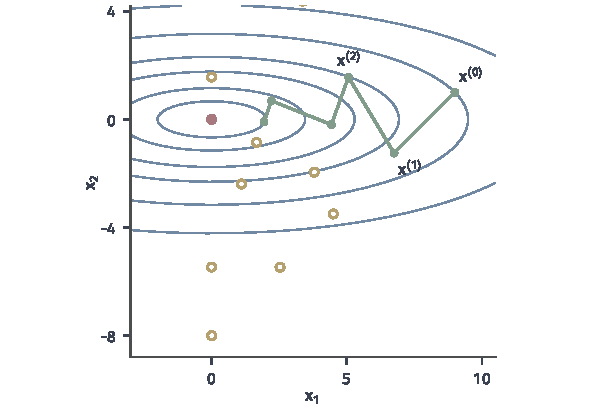
\includegraphics[width=100mm]{figures/05-optimization/02-smooth-optimization/matplotlib/smooth-backtrack-path/figure.pdf}
  \caption{回溯的路径。绿点和绿线是前五轮接受的点，黄色空心点是这几轮被拒绝的试探点，它们都落在比当前点差得多的位置，超出图幅的未画出。目标见例~\eqref{eq:smooth-running}，参数同表~\ref{tab:smooth-backtrack-run}。}
  \label{fig:smooth-backtrack-path}
\end{BookInlineFigure}

从$t=3$起步长在$0.5$与$0.125$之间交替：沿平坦方向时能迈大步，碰到陡峭分量时又缩回来。迭代在$\lVert\bm{g}\rVert_2\leq10^{-3}$时结束，共$25$轮、$76$次试探。最终得到
\[
 \bm{x}^{(25)}\approx(4.98\times10^{-4},\,-2.2\times10^{-5}),\qquad f(\bm{x}^{(25)})\approx1.3\times10^{-7}.
\]

\paragraph{每次试探增加的函数计算}
回溯的代价是被拒绝的试探。一轮共试探$n$次，就多算$n$次函数值。由式~\eqref{eq:smooth-backtracking-bounds}，例中第一轮的$\bar{\alpha}=0.2$，试探次数的上界是$1+\lceil\log_25\rceil=4$，实际是$3$次。

每轮都从同一个$\alpha_0$开始，就要反复支付同样的试探。一个自然的办法是用上一轮接受的步长作起点，也就是$\alpha_0^{(t+1)}=\alpha^{(t)}$。这时步长不增，设$\nabla f$全局$L$光滑、方向为负梯度，则每次拒绝都发生在$\alpha>\bar{\alpha}=2(1-c_1)/L$的步长上。每次拒绝让步长缩小$\rho$倍，所以全程被拒绝的总次数$R$满足
\begin{equation}
 R\leq1+\log_{1/\rho}\frac{\alpha_0L}{2(1-c_1)}.
 \label{eq:smooth-total-rejections}
\end{equation}
这样，函数计算的总次数是$T+R$，也就是只比轮数多一个对数项。例中上界约是$3.3$，全程实际拒绝$3$次。

但是步长只减不增，走到平坦的区域也不能放大。折中的办法是每轮把初值放大$1/\rho$倍。取$\rho=1/2$时，第$t$轮被拒绝$r_t$次，步长变化是
\[
 \alpha^{(t+1)}=2\cdot2^{-r_{t+1}}\alpha^{(t)}.
\]
累加后，只要步长有正的下界，$\sum_tr_t$至多比$T$多一个常数，所以每轮平均约试探两次。图~\ref{fig:smooth-backtrack-cost}中，每轮从$1$开始时平均$3.04$次，放大策略平均$2.06$次。

\begin{BookInlineFigure}
  \centering
  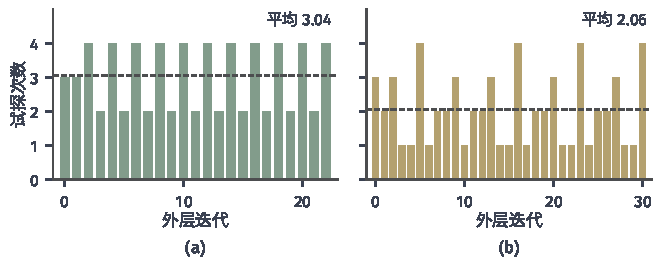
\includegraphics[width=112mm]{figures/05-optimization/02-smooth-optimization/matplotlib/smooth-backtrack-cost/figure.pdf}
  \caption{每轮的试探次数，直到目标差不超过$10^{-6}$，目标见例~\eqref{eq:smooth-running}。(a)每轮都从$\alpha_0=1$开始，共$23$轮、$70$次试探。(b)每轮的初值取上一轮接受步长的$2$倍，共$31$轮、$64$次试探。虚线是平均值。}
  \label{fig:smooth-backtrack-cost}
\end{BookInlineFigure}

试探的单价也可以压低。例如最小二乘$\frac12\lVert\bm{A}\bm{x}-\bm{b}\rVert_2^2$，只要算一次$\bm{A}\bm{d}$，每个候选的目标值就是$\frac12\lVert\bm{r}+\alpha\bm{A}\bm{d}\rVert_2^2$，其中$\bm{r}=\bm{A}\bm{x}-\bm{b}$，只需向量运算。通过的试探点的函数值和部分中间量也常能在计算下一轮梯度时复用。

\subsection{Wolfe条件}
\label{sec:smooth-wolfe}

\paragraph{只看函数值挡不住太小的步长}
Armijo条件只限制步长不能太大，太小的步长总能通过。回溯之所以没有这个问题，是因为被接受的步长的上一次试探失败过，$\alpha$不会比门槛小太多。可一旦步长不是由回溯产生，比如来自插值或其他公式，这层保护就没有了。

下面的例子中，每一步都满足Armijo条件，迭代却停在非驻点。取$f(x)=x^2$，方向恒为$d=-1$，步长$\alpha^{(t)}=2^{-t-1}$，于是
\[
 x^{(t)}=1+2^{-t}\to1.
\]

一步的实际下降量和预测下降量分别是
\[
 2^{-t-1}\bigl(2+3\cdot2^{-t-1}\bigr),\qquad 2^{-t-1}\bigl(2+2^{1-t}\bigr).
\]
括号比较可知，$c_1\leq3/4$时Armijo条件每一步都成立。但极限点$x=1$处$f'(1)=2\neq0$，迭代不是因为到了谷底才停下，只是步子缩得太快。图~\ref{fig:smooth-short-steps}(a)画出了这个序列。

\begin{BookInlineFigure}
  \centering
  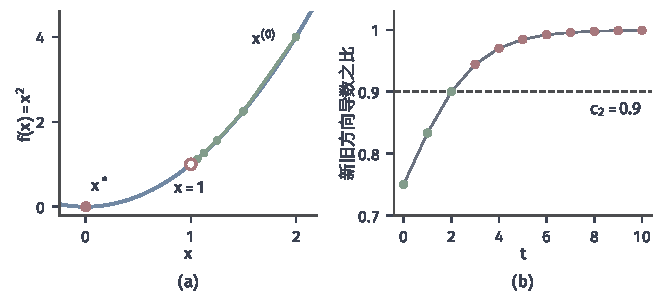
\includegraphics[width=112mm]{figures/05-optimization/02-smooth-optimization/matplotlib/smooth-short-steps/figure.pdf}
  \caption{只满足Armijo条件的序列可能停在非驻点。(a)$f(x)=x^2$上的序列$x^{(t)}=1+2^{-t}$（绿点），收敛到空心红点$x=1$，真正的最优解是实心红点。(b)每步新旧方向导数之比。比值超过虚线$c_2=0.9$的点（红色）不满足曲率条件。}
  \label{fig:smooth-short-steps}
\end{BookInlineFigure}

\paragraph{用斜率判断“还能走”}
步子太短的后果，可以从落脚点的坡度看出来。如果落脚后$\phi'(\alpha)$仍然和$\phi'(0)$差不多陡，说明继续往前走还有几乎同样的下降率，停下来可惜。反之，坡度已经明显变缓甚至变正，才说明这段路的收益基本取尽了。用上面的例子算比值：
\[
 \frac{\phi'(\alpha^{(t)})}{\phi'(0)}=\frac{2+2^{-t}}{2+2^{1-t}}\to1.
\]
落脚点的坡度几乎不变，这正是步长太短的标志，见图~\ref{fig:smooth-short-steps}(b)。

\begin{definition}[Wolfe条件]
\label{def:smooth-wolfe}
设$\langle\bm{g},\bm{d}\rangle<0$，$0<c_1<c_2<1$。若$\alpha>0$满足Armijo条件~\eqref{eq:smooth-armijo}和
\begin{equation}
 \langle\nabla f(\bm{x}+\alpha\bm{d}),\bm{d}\rangle\geq c_2\langle\bm{g},\bm{d}\rangle,
 \label{eq:smooth-curvature}
\end{equation}
就说它满足\term{Wolfe条件}（Wolfe conditions）；式~\eqref{eq:smooth-curvature}单独称为\term{曲率条件}（curvature condition）。若把式~\eqref{eq:smooth-curvature}换成
\begin{equation}
 \bigl\lvert\langle\nabla f(\bm{x}+\alpha\bm{d}),\bm{d}\rangle\bigr\rvert\leq c_2\lvert\langle\bm{g},\bm{d}\rangle\rvert,
 \label{eq:smooth-strong-curvature}
\end{equation}
就说它满足\term{强Wolfe条件}（strong Wolfe conditions）。
\end{definition}

曲率条件只限制方向导数不能太负，也就是挡住太短的步长；Armijo条件挡住太长的步长；两者一上一下。强条件还限制方向导数不能太正，因而在最低点附近形成一个窗口。

在二次目标上，由式~\eqref{eq:smooth-quadratic-line}，方向导数之比是$1-\alpha/\alpha_{\mathrm{e}}$，两种条件的区间可以直接写出：
\begin{equation}
 \begin{aligned}
 \text{Wolfe：}&\quad(1-c_2)\alpha_{\mathrm{e}}\leq\alpha\leq2(1-c_1)\alpha_{\mathrm{e}},\\
 \text{强Wolfe：}&\quad(1-c_2)\alpha_{\mathrm{e}}\leq\alpha\leq\min\{1+c_2,\,2(1-c_1)\}\alpha_{\mathrm{e}}.
 \end{aligned}
 \label{eq:smooth-wolfe-quadratic}
\end{equation}

例~\eqref{eq:smooth-running}第一轮，$\alpha_{\mathrm{e}}=0.2$，取$c_1=0.1$，$c_2=0.5$。Wolfe区间是$[0.1,0.36]$，强Wolfe区间是$[0.1,0.3]$。代入三个候选步长检验，其中$c_2\phi'(0)=-81$：
\[
 \begin{aligned}
 \alpha=0.05:&\quad\phi'=-121.5<-81,\ \text{太短，不通过};\\
 \alpha=0.25:&\quad\phi'=40.5,\ \text{两种条件都通过};\\
 \alpha=0.33:&\quad\phi'=105.3,\ \text{Wolfe通过，强Wolfe不通过}.
 \end{aligned}
\]

图~\ref{fig:smooth-wolfe-intervals}换了一个非凸的一元剖面。Armijo条件的可接受集是一个长区间；加上曲率条件后，靠近$0$的太短步长被去掉；强条件再去掉斜率太大的部分，只留下每个谷底、谷间凸起附近的小窗口。这里的窗口不止一个，线搜索只需要落进其中之一。

\begin{BookInlineFigure}
  \centering
  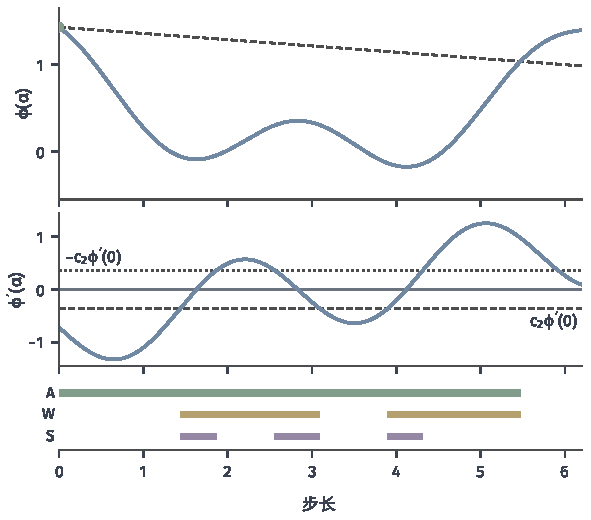
\includegraphics[width=100mm]{figures/05-optimization/02-smooth-optimization/matplotlib/smooth-wolfe-intervals/figure.pdf}
  \caption{非凸剖面$\phi(\alpha)=0.12(\alpha-3)^2+0.35\cos(2.2\alpha)$上的可接受步长，$c_1=0.1$，$c_2=0.5$。上图虚线是Armijo检验直线，中图的虚线和点线是$\pm c_2\phi'(0)$。下方三条：A是满足Armijo条件的步长，W是满足Wolfe条件的步长，S是满足强Wolfe条件的步长。}
  \label{fig:smooth-wolfe-intervals}
\end{BookInlineFigure}

\paragraph{满足条件的步长存在}
要使用这些条件，先要确认可接受的步长总是存在。需要的额外假设是$\phi$有下界；否则沿这条线可以无限下降，不存在要停下的理由。

\begin{theorem}[Wolfe步长的存在]
\label{thm:smooth-wolfe-existence}
设$f$连续可微，$\langle\bm{g},\bm{d}\rangle<0$，$\phi$在$[0,\infty)$上有下界，$0<c_1<c_2<1$。则存在一个开区间，其中每个步长都满足强Wolfe条件，因而也满足Wolfe条件。
\end{theorem}

\begin{proof}
直线$\ell(\alpha)=\phi(0)+c_1\alpha\phi'(0)$无下界，而$\phi$有下界，所以两者在某个正步长相交。因$\phi'(0)<c_1\phi'(0)$，$\alpha$很小时$\phi<\ell$。记最小的正交点为$\alpha'$，于是在$(0,\alpha')$上$\phi<\ell$。

由微分中值定理，存在$\alpha''\in(0,\alpha')$，使
\[
 \phi'(\alpha'')=\frac{\phi(\alpha')-\phi(0)}{\alpha'}=c_1\phi'(0).
\]

因为$0<c_1<c_2$且$\phi'(0)<0$，$\alpha''$处同时有
\[
 \phi'(\alpha'')>c_2\phi'(0),\qquad \lvert\phi'(\alpha'')\rvert<c_2\lvert\phi'(0)\rvert.
\]
$\phi'$连续，这两个严格不等式在$\alpha''$的一个邻域内保持；邻域取得足够小时留在$(0,\alpha')$中，Armijo条件也严格成立。
\end{proof}

定理保证了存在，算法还要把这样的步长找出来。满足Wolfe条件的一个简单办法是二分。维护区间$[\alpha_{\mathrm{lo}},\alpha_{\mathrm{hi}}]$，初值为$[0,\infty)$，用一个试探点$\alpha$：Armijo不满足，就令$\alpha_{\mathrm{hi}}=\alpha$；Armijo满足而曲率条件不满足，就令$\alpha_{\mathrm{lo}}=\alpha$；两者都满足则接受。新试探点取区间中点，上端还是无穷时取$2\alpha_{\mathrm{lo}}$。

这个过程有限步终止。假如一直不停，且$\alpha_{\mathrm{hi}}$始终是无穷，则$\alpha_{\mathrm{lo}}\to\infty$且都满足Armijo条件，推出$\phi\to-\infty$，与下界矛盾。

否则区间缩到一点$\alpha_\infty$。由端点的Armijo状态，$\phi(\alpha_{\mathrm{hi}})$在直线上方，$\phi(\alpha_{\mathrm{lo}})$在直线下方，两者作差商后取极限，得到$\phi'(\alpha_\infty)\geq c_1\phi'(0)$。另一方面$\alpha_{\mathrm{lo}}$不满足曲率条件，取极限得到$\phi'(\alpha_\infty)\leq c_2\phi'(0)$。于是
\[
 c_1\phi'(0)\leq\phi'(\alpha_\infty)\leq c_2\phi'(0).
\]
而$c_1<c_2$、$\phi'(0)<0$说明$c_2\phi'(0)<c_1\phi'(0)$，矛盾。

用例子走两次。从$\alpha=1$开始时，$1$和$0.5$都不满足Armijo条件，上端缩到$0.5$，试探$0.25$，两个条件都满足，接受。从$\alpha=0.05$开始时，Armijo满足，曲率条件不满足，下端更新为$0.05$，上端还是无穷，试探$0.1$，它恰好落在Wolfe区间的左端点上，接受。强Wolfe条件要用更细致的分段放大与缩小程序，每轮通常只需很少几次试探，具体写法可查阅\scite{math-nocedal2006numerical}。

\paragraph{Wolfe条件怎样避免步长过小}
下面的定理把“不会太小”写成定量结论，并给出它累积起来的效果。这里只要求当前点和接受点之间满足Lipschitz条件。

\begin{theorem}[Wolfe步长的下界与累积下降]
\label{thm:smooth-wolfe-decrease}
设步长$\alpha$满足Wolfe条件，$\bm{x}$与$\bm{x}+\alpha\bm{d}$这一对点满足以$L$为常数的式~\eqref{eq:smooth-lipschitz}。则
\begin{equation}
 \alpha\geq\frac{(1-c_2)\lvert\langle\bm{g},\bm{d}\rangle\rvert}{L\lVert\bm{d}\rVert_2^2},
 \label{eq:smooth-wolfe-lower}
\end{equation}
\begin{equation}
 f(\bm{x})-f(\bm{x}+\alpha\bm{d})\geq\frac{c_1(1-c_2)}{L}\cos^2\theta\,\lVert\bm{g}\rVert_2^2,
 \label{eq:smooth-wolfe-decrease}
\end{equation}
其中$\theta$是$\bm{d}$与$-\bm{g}$的夹角。若$f$下有界，且迭代的每一步都满足上述假设，则
\begin{equation}
 \sum_{t=0}^{\infty}\cos^2\theta^{(t)}\,\lVert\bm{g}^{(t)}\rVert_2^2<\infty.
 \label{eq:smooth-zoutendijk}
\end{equation}
\end{theorem}

\begin{proof}
从曲率条件~\eqref{eq:smooth-curvature}两端减去$\langle\bm{g},\bm{d}\rangle$，得到
\[
 \langle\nabla f(\bm{x}+\alpha\bm{d})-\bm{g},\bm{d}\rangle\geq(c_2-1)\langle\bm{g},\bm{d}\rangle=(1-c_2)\lvert\langle\bm{g},\bm{d}\rangle\rvert.
\]

由Cauchy--Schwarz不等式和假设，左端不超过$L\alpha\lVert\bm{d}\rVert_2^2$，于是式~\eqref{eq:smooth-wolfe-lower}成立。

把式~\eqref{eq:smooth-wolfe-lower}代入Armijo条件~\eqref{eq:smooth-armijo}，一步下降量不小于
\[
 c_1\alpha\lvert\langle\bm{g},\bm{d}\rangle\rvert\geq\frac{c_1(1-c_2)}{L}\cdot\frac{\langle\bm{g},\bm{d}\rangle^2}{\lVert\bm{d}\rVert_2^2},
\]
再由$\cos\theta$的定义，即得式~\eqref{eq:smooth-wolfe-decrease}。

对$t=0,\ldots,T-1$累加，左端不超过$f(\bm{x}^{(0)})-\inf f$，与$T$无关。令$T\to\infty$，式~\eqref{eq:smooth-zoutendijk}成立。
\end{proof}

式~\eqref{eq:smooth-zoutendijk}称为\term{Zoutendijk条件}（Zoutendijk condition）。它把线搜索和方向分开：线搜索保证了这个级数收敛，方向只需不要越来越贴近等高线。若$\cos\theta^{(t)}\geq\delta>0$一直成立，就有$\lVert\bm{g}^{(t)}\rVert_2\to0$。回到图~\ref{fig:smooth-short-steps}的序列：那里$\cos\theta^{(t)}=1$，梯度却不趋于零，它违反的正是曲率条件。

下降量~\eqref{eq:smooth-wolfe-decrease}和式~\eqref{eq:smooth-cos-decrease}形式相同，只是常数不同。这说明Wolfe条件在不知道$L$的情况下，达到了和按$L$选步长同量级的保证。

\paragraph{拟牛顿曲率更新中的用途}
第~\ref{chap:quasi-newton}章的方法用相邻两点的梯度差来逼近曲率。设相邻两点的位移和梯度差是
\[
 \bm{s}=\alpha\bm{d},\qquad \bm{y}=\nabla f(\bm{x}+\alpha\bm{d})-\bm{g}.
\]
若要让对称正定矩阵$\bm{B}$满足$\bm{B}\bm{s}=\bm{y}$，两边与$\bm{s}$作内积，就得到必要条件
\[
 \langle\bm{s},\bm{y}\rangle=\langle\bm{s},\bm{B}\bm{s}\rangle>0.
\]

这个条件对非凸目标不会自动成立，而Wolfe条件恰好保证它。由曲率条件，
\begin{equation}
 \langle\bm{s},\bm{y}\rangle=\alpha\bigl(\phi'(\alpha)-\phi'(0)\bigr)\geq\alpha(1-c_2)\lvert\phi'(0)\rvert>0.
 \label{eq:smooth-wolfe-curvature-pair}
\end{equation}
这里只需要Wolfe条件，不需要强Wolfe条件。

用$f(x)=1-\cos x$、$x=2$、$d=-1$看两个步长，取$c_1=0.1$，$c_2=0.9$。此时$\phi'(0)=-\sin2\approx-0.909$。图~\ref{fig:smooth-secant-curvature}中，黄线和绿线对应下面的两个候选：
\[
 \begin{aligned}
 \alpha=0.4:&\quad\phi'(\alpha)\approx-1.000,\quad\langle\bm{s},\bm{y}\rangle\approx-0.036,\\
 \alpha=1.3:&\quad\phi'(\alpha)\approx-0.644,\quad\langle\bm{s},\bm{y}\rangle\approx0.345.
 \end{aligned}
\]
两者都满足Armijo条件。$\alpha=0.4$不满足曲率条件，得到的$\langle\bm{s},\bm{y}\rangle$是负的，不能用来更新正定矩阵；$\alpha=1.3$满足Wolfe条件，可以使用。

\begin{BookInlineFigure}
  \centering
  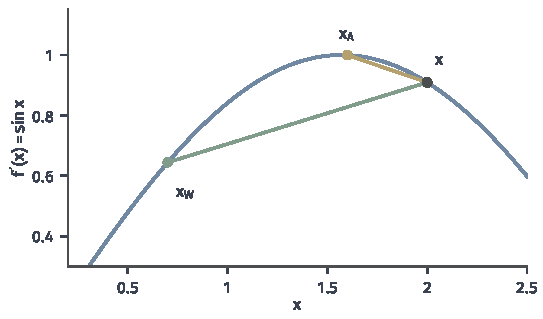
\includegraphics[width=92mm]{figures/05-optimization/02-smooth-optimization/matplotlib/smooth-secant-curvature/figure.pdf}
  \caption{曲率条件与割线斜率。蓝线是$f(x)=1-\cos x$的导数$\sin x$，深灰点是当前点$x=2$，沿$d=-1$移动。黄点$x_{\mathrm{A}}=1.6$只满足Armijo条件，割线斜率$y/s$为负。绿点$x_{\mathrm{W}}=0.7$满足Wolfe条件，割线斜率为正。}
  \label{fig:smooth-secant-curvature}
\end{BookInlineFigure}

\paragraph{非线性共轭梯度的下降分析中的用途}
强Wolfe条件的用处在另一类方法。第~\ref{chap:first-order-methods}章的非线性共轭梯度法把新方向取成新的负梯度加上旧方向的倍数。下面记新点的梯度为$\bm{g}_+$，系数为$\beta$：
\[
 \bm{d}_+=-\bm{g}_++\beta\bm{d}.
\]

新方向要是下降方向，需要检查它的方向导数：
\begin{equation}
 \langle\bm{g}_+,\bm{d}_+\rangle=-\lVert\bm{g}_+\rVert_2^2+\beta\langle\bm{g}_+,\bm{d}\rangle.
 \label{eq:smooth-cg-descent}
\end{equation}
第二项中的$\langle\bm{g}_+,\bm{d}\rangle$恰好是上一轮落脚点的方向导数。它若太大，加上$\beta$的放大可能抵消第一项，新方向就不再下降。Wolfe条件只限制它不能太负，对正的一侧不设限；强Wolfe条件才限制它的绝对值。

图~\ref{fig:smooth-cg-descent}用具体的向量说明差别。取$\bm{g}=(2,0)$，$\bm{d}=-\bm{g}$，系数取一种常见形式：
\[
 \beta=\frac{\lVert\bm{g}_+\rVert_2^2}{\lVert\bm{g}\rVert_2^2}.
\]

\begin{BookInlineFigure}
  \centering
  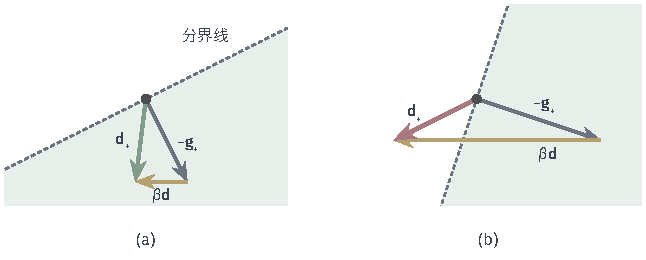
\includegraphics[width=108mm]{figures/05-optimization/02-smooth-optimization/tikz/smooth-cg-descent/figure.pdf}
  \caption{落脚点的方向导数决定新方向是否下降。浅绿区域是$\bm{g}_+$对应的下降半平面，虚线是分界线。旧方向$\bm{d}=(-2,0)$，灰色箭头是$-\bm{g}_+$，黄色箭头是$\beta\bm{d}$，两者之和是$\bm{d}_+$。(a)$\bm{g}_+=(-0.5,1)$，$\langle\bm{g}_+,\bm{d}\rangle=1$，绿色的$\bm{d}_+$留在半平面内。(b)$\bm{g}_+=(-3,1)$，$\langle\bm{g}_+,\bm{d}\rangle=6$，超过$\lvert\langle\bm{g},\bm{d}\rangle\rvert=4$，红色的$\bm{d}_+$落到半平面之外。}
  \label{fig:smooth-cg-descent}
\end{BookInlineFigure}

两种情形的数值分别是
\[
 \begin{aligned}
 \bm{g}_+=(-0.5,1):&\quad\beta=0.3125,\quad\langle\bm{g}_+,\bm{d}_+\rangle=-0.9375,\\
 \bm{g}_+=(-3,1):&\quad\beta=2.5,\quad\langle\bm{g}_+,\bm{d}_+\rangle=5.
 \end{aligned}
\]
后一种情形的新方向是上升方向。强Wolfe条件取$c_2<1$就排除了这种比值大于$1$的情况；要在所有轮次都保证下降，还需要对$c_2$的进一步限制和相应的$\beta$公式，这些在第~\ref{chap:first-order-methods}章讨论。常用参数也反映了这种分工：拟牛顿法常取$c_2=0.9$，非线性共轭梯度常取$c_2=0.1$\scite{math-nocedal2006numerical}。

\paragraph{精确线搜索：只作理论对照}
把窗口一直收紧，就得到\term{精确线搜索}（exact line search）：取$\phi$的最小点，至少满足
\begin{equation}
 \langle\nabla f(\bm{x}+\alpha\bm{d}),\bm{d}\rangle=0.
 \label{eq:smooth-exact-orthogonal}
\end{equation}
这是$c_2\to0$时强Wolfe条件的极限。此时式~\eqref{eq:smooth-cg-descent}的第二项消失，分析变得干净，所以理论推导常先考虑它。

二次目标上式~\eqref{eq:smooth-exact-quadratic}给出显式解。例~\eqref{eq:smooth-running}用精确步长，从形如$r(9,\pm1)$的点出发，一步到达$0.8r(9,\mp1)$，所以
\[
 \bm{x}^{(t)}=0.8^t\bigl(9,(-1)^t\bigr).
\]
下一轮的方向是下一轮的负梯度，式~\eqref{eq:smooth-exact-orthogonal}说明相邻方向互相垂直，于是路径成直角锯齿，如图~\ref{fig:smooth-exact-zigzag}。

\begin{BookInlineFigure}
  \centering
  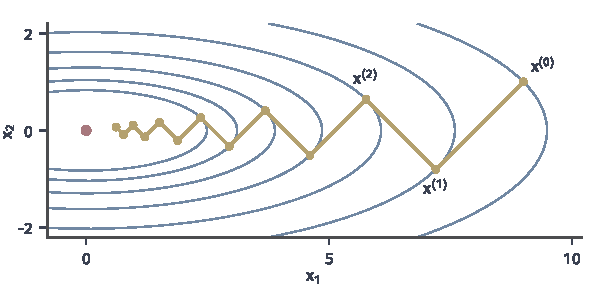
\includegraphics[width=100mm]{figures/05-optimization/02-smooth-optimization/matplotlib/smooth-exact-zigzag/figure.pdf}
  \caption{精确线搜索的路径。黄点是例~\eqref{eq:smooth-running}上负梯度方向取精确步长的迭代点，蓝线是经过这些点的等高线。每一段都在终点与等高线相切，相邻两段互相垂直，目标每轮乘以$0.64$。}
  \label{fig:smooth-exact-zigzag}
\end{BookInlineFigure}

“精确”并不等于最好。这个例子上精确线搜索每轮目标缩小到$0.64$倍，而下一节会看到，回溯用更少的轮数就达到了同样的精度。对一般目标，精确求解一维问题要多次函数或梯度计算，非凸时还要说明找的是哪个局部最小点。因此实际算法使用有限的接受条件，精确线搜索只作为分析时的对照。

\paragraph{三种规则的比较}
表~\ref{tab:smooth-step-rules}汇总本节的比较。比较的对象都是沿固定下降方向选步长，差别在事先要什么信息、每轮多算什么、换来什么保证。

\begin{table*}[!htbp]
  \centering
  \begin{tabular}{@{}llll@{}}
    \toprule
    规则 & 事先需要 & 每轮额外计算 & 保证\\
    \midrule
    固定步长 & $L$的上界，方向的尺度 & 无 & 式~\eqref{eq:smooth-gd-step}、\eqref{eq:smooth-cos-decrease}\\
    回溯（Armijo） & 下降方向，初始试探步长 & $n$次函数值 & 式~\eqref{eq:smooth-backtracking-decrease}\\
    Wolfe & $\phi$有下界 & 函数值和方向导数 & 式~\eqref{eq:smooth-wolfe-decrease}，$\langle\bm{s},\bm{y}\rangle>0$\\
    强Wolfe & 同上 & 同上，试探常更多 & 另限制落脚点方向导数的绝对值\\
    精确线搜索 & $\phi$的最小点可求 & 一维优化 & 落脚点方向导数为零\\
    \bottomrule
  \end{tabular}
  \caption{选择步长的规则。各行的保证都针对固定的下降方向，方向的质量由夹角$\theta$单独体现。}
  \label{tab:smooth-step-rules}
\end{table*}
